% !TEX root = ../main.tex
\section{Phân tích lỗi}\label{sec:error}

Bộ phát hiện hoạt động tốt; các vấn đề tập trung ở khâu nhận dạng và ở dữ liệu. Phân tích chỉ ra ba nguyên nhân độc lập.

\subsection{Khoảng cách miền của bộ nhận dạng}
\paragraph{Tình huống \code{54-L1 9999}.} Hình~\ref{fig:case} là một ảnh chụp thật. Với phiên bản CRNN đầu tiên, chuỗi đọc được là \code{5HL1}: số \code{4} bị đọc thành \code{H}. Lần theo pipeline cho thấy bộ phát hiện (độ tin cậy 0,85), phân loại 2 dòng và tách dòng đều đúng; lỗi nằm hoàn toàn ở CRNN. Trong font Hershey dùng để sinh dữ liệu, số \code{4} có đỉnh khép kín, còn trong font biển số Việt Nam, số \code{4} hở đỉnh và rất giống chữ \code{H}. Phân tích xác suất đầu ra cho thấy ở vị trí đó mô hình gần như đoán mò (\code{Z}, \code{V}, \code{L} cùng khoảng 0,2), nhưng nếu chỉ xét các chữ số thì \code{4} vẫn trội hẳn (0,13 so với 0,005). Phiên bản CRNN đang dùng đọc đúng ảnh này với độ tin cậy 98,6\,\%.

\begin{figure}[H]
\centering
\begin{subfigure}[b]{0.48\linewidth}
  \centering
  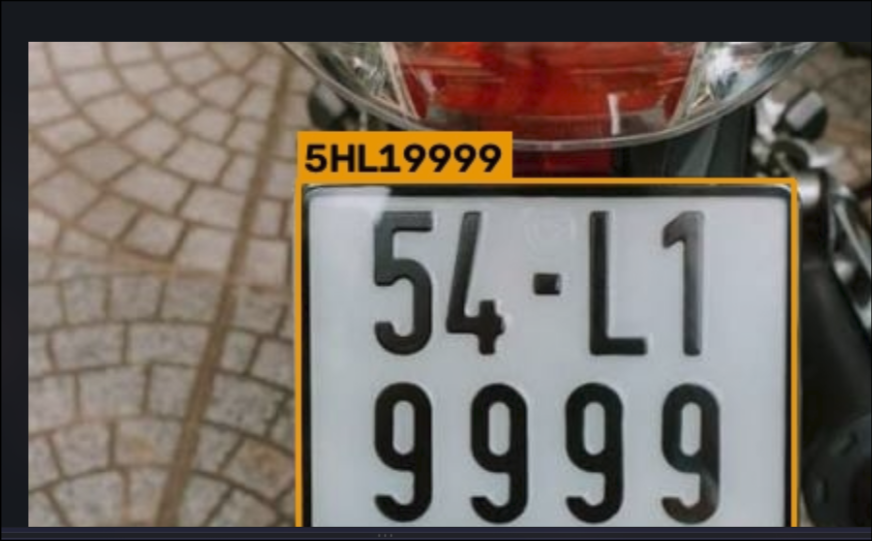
\includegraphics[width=\linewidth]{figures/case_54L1.png}
  \caption{Ảnh chụp thật (khung do bộ phát hiện vẽ).}
\end{subfigure}\hfill
\begin{subfigure}[b]{0.48\linewidth}
  \centering
  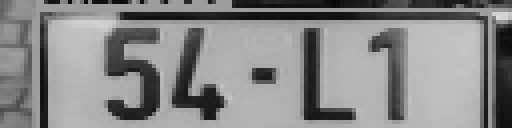
\includegraphics[width=\linewidth]{figures/case_line1.png}\\[0.4em]
  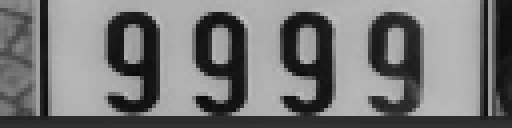
\includegraphics[width=\linewidth]{figures/case_line2.png}
  \caption{Hai ảnh dòng chữ CRNN nhận được ($32\times128$, phóng to).}
\end{subfigure}
\caption{Tình huống \code{54-L1 9999}: phiên bản CRNN đầu đọc thành \code{5HL1}, phiên bản hiện tại đọc đúng.}
\label{fig:case}
\end{figure}

\paragraph{Trên bộ dữ liệu.} Tuy đọc đúng ảnh cận cảnh rõ nét, CRNN không đọc đúng biển nào trong 154 biển của tập test (Bảng~\ref{tab:real}), trong khi đạt 95,7\,\% trên biển tổng hợp. Ảnh cắt trong bộ dữ liệu khác dữ liệu tổng hợp ở nhiều mặt cùng lúc: độ phân giải thấp, font biển thật, chữ bị co hẹp do ảnh bị co giãn (Mục~\ref{sec:two-line}), cùng bóng đổ, ốc vít và khung biển. Mô hình chỉ học trên dữ liệu tổng hợp nên học thuộc hình dạng của font Hershey thay vì học đặc trưng chung của chữ số. Đây là \textbf{điểm nghẽn chính} của hệ thống.

\subsection{Phân loại 1 dòng / 2 dòng bằng tỉ lệ khung}\label{sec:two-line}
Pipeline coi một ảnh cắt là biển 2 dòng khi tỉ lệ rộng/cao nhỏ hơn 2,5, dựa trên giả định biển ô tô 1 dòng có tỉ lệ khoảng 4,7:1. Trên tập test, giả định này không còn đúng:

\begin{table}[H]
\centering
\caption{Tỉ lệ rộng/cao của ảnh cắt biển trong tập test và kết quả phân loại với ngưỡng 2,5.}
\label{tab:aspect}
\begin{tabular}{lrrr}
\toprule
Loại biển (theo nhãn) & Số biển & Trung vị rộng/cao & Bị coi là 2 dòng \\
\midrule
1 dòng & 98 & 2,08 & 70 (71\,\%) \\
2 dòng & 205 & 1,08 & 205 (100\,\%) \\
\bottomrule
\end{tabular}
\end{table}

Biển 1 dòng chỉ còn tỉ lệ khoảng 2:1, thấp hơn nhiều so với kích thước thật. Nhiều khả năng ảnh trong bộ dữ liệu đã bị co giãn về $640\times640$ khi xuất từ Roboflow, làm biển bị bóp hẹp theo chiều ngang. Hệ quả là 71\,\% biển 1 dòng bị cắt đôi trước khi đưa vào OCR, làm hỏng kết quả của cả CRNN lẫn bản nháp của PaddleOCR. Đặt ngưỡng cố định theo kích thước biển thật là không đủ an toàn; cách phân loại cần dựa vào chính nội dung ảnh (Mục~\ref{sec:limit}).

\subsection{Chất lượng nhãn chữ}\label{sec:labels-quality}
Toàn bộ 303 nhãn được đánh dấu ``đã duyệt'' của tập test \textbf{trùng khớp hoàn toàn} với bản nháp của PaddleOCR, và chỉ 154 nhãn trong số đó là biển số hợp lệ. Nhìn vào ảnh cắt có thể thấy nhãn sai rõ ràng (Hình~\ref{fig:labels}): biển \code{51A-775.29} được gán \code{00/51A77529}, biển \code{51A-052.27} được gán \code{51A05227/JTAUSEILA}. Những nhãn này đến từ chính lỗi tách dòng ở Mục~\ref{sec:two-line}: PaddleOCR đọc từng nửa biển và trả về cả các ký tự rác.

\begin{figure}[H]
\centering
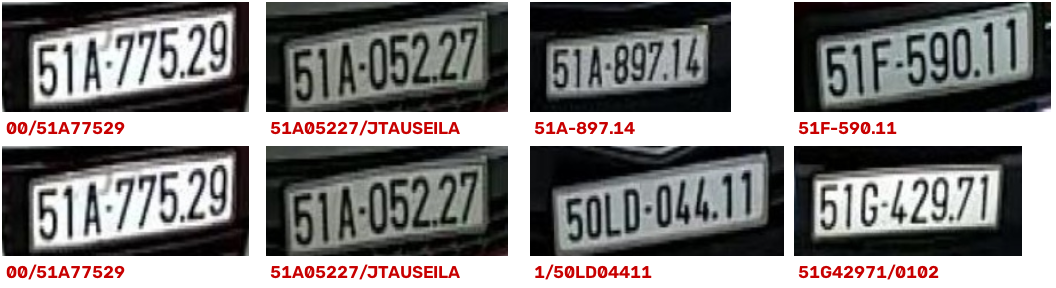
\includegraphics[width=\linewidth]{figures/test_label_samples.png}
\caption{Ảnh cắt biển trong tập test và nhãn đang có (chữ đỏ). Nhãn là bản nháp của PaddleOCR, chưa được sửa.}
\label{fig:labels}
\end{figure}

Bài học rút ra là bước duyệt nhãn phải thật sự là người kiểm tra từng ảnh, đặc biệt với tập test: một tập đáp án sinh ra từ một mô hình sẽ làm mọi phép so sánh thiên vị về phía mô hình đó.

\subsection{Nhận xét chung}
\begin{itemize}[nosep]
  \item Bộ phát hiện đạt chỉ tiêu và không phải là điểm nghẽn.
  \item Độ chính xác trên dữ liệu tổng hợp \emph{không} phản ánh độ chính xác thật; đánh giá trên ảnh thật với nhãn đã duyệt là bắt buộc.
  \item Ba vấn đề cộng dồn với nhau: lỗi tách dòng làm hỏng bản nháp, nhãn hỏng chưa được sửa, và CRNN chưa từng thấy biển thật. Sửa theo đúng thứ tự (phân loại dòng, duyệt nhãn, rồi fine-tune) mới tránh được việc huấn luyện trên dữ liệu sai.
\end{itemize}
